\documentclass[11pt]{article}
\usepackage[T1]{fontenc}
\usepackage{lmodern,amsmath,amssymb,amsthm,microtype,booktabs,array,xcolor,graphicx,tikz}
\usepackage[margin=1.1in]{geometry}
\usepackage[font=small,labelfont=bf,skip=8pt]{caption}
\usepackage{url}
\makeatletter\g@addto@macro{\UrlBreaks}{\do\a\do\b\do\c\do\d\do\e\do\f\do\g\do\h\do\i\do\j\do\k\do\l\do\m\do\n\do\o\do\p\do\q\do\r\do\s\do\t\do\u\do\v\do\w\do\x\do\y\do\z\do\0\do\1\do\2\do\3\do\4\do\5\do\6\do\7\do\8\do\9\do\-}\makeatother
\usepackage[colorlinks=true,linkcolor=blue!50!black,citecolor=green!35!black,urlcolor=blue!50!black]{hyperref}
\newtheorem{theorem}{Theorem}
\newtheorem{lemma}{Lemma}
\newcommand{\val}{\mathrm{val}}
\newcommand{\lean}[1]{\texttt{#1}}
\setlength{\emergencystretch}{3em}
\hypersetup{pdftitle={Uncrossing Wires for 3-SAT: A Potential That Closes the Recursion},pdfauthor={Siyuan Zhuang}}

\title{Uncrossing Wires for 3-SAT:\\A Potential That Closes the Recursion}
\author{Siyuan Zhuang}
\date{October 31, 2026}

\begin{document}
\maketitle

\begin{abstract}
We prove that for each $\varepsilon>0$, 3-SAT with $n$ variables can be decided by a deterministic algorithm in time $C_\varepsilon|\varphi|^{O_\varepsilon(1)}2^{\varepsilon n}$, where $|\varphi|$ is the size of the input. So the Exponential Time Hypothesis fails. OpenAI and Claude (Anthropic) first announced this statement. Our proof has these features. Besides the branching that reduces the occurrences of a variable, it is elementary: one identity on four bits, a count of strings, and the Cauchy--Schwarz inequality. It has no polynomial approximation, no spectral argument and no determinant. It is a recursion on one fixed tower of grids, with two pieces for each rectangle, and with no regrouping of nodes.

The main finding is a measure that closes the recursion. View a formula as a network: nodes on a grid, joined by wires that each hold a bit. The number of wires need not fall from one level of the recursion to the next: a rectangle with wires on only one diagonal keeps all of them. But those wires then occupy fewer pairs of nodes, and a quadratic potential sees this. It falls by the fixed factor $\sqrt{24/25}$ for every term, in one of the two directions, whatever the weights are. So weights need not be balanced, and one short inequality closes the recursion. Two wires that cross both the rows and the columns of a grid are replaced by two terms, each crossing only one of them; a choice of terms gives a network on the rows or on the columns; and we keep the one with the smaller potential. The theorem is formalized in Lean~4 down to a multitape machine, with its time and space.
\end{abstract}

\section*{The result and the strategy}

\begin{theorem}\label{thm:sat}
For each $\varepsilon>0$, 3-SAT with $n$ variables is decided deterministically in time $C_\varepsilon|\varphi|^{O_\varepsilon(1)}2^{\varepsilon n}$, where $|\varphi|$ is the size of the input $\varphi$.
\end{theorem}

The Exponential Time Hypothesis of Impagliazzo and Paturi~\cite{IP01} says that for some $\delta>0$, no algorithm decides 3-SAT on $n$ variables in time $2^{\delta n}$ times a polynomial in the input size. Theorem~\ref{thm:sat} contradicts this: take $\varepsilon<\delta$. The degree of the polynomial may depend on $\varepsilon$; after duplicates are removed the input has size polynomial in $n$.

\subsection*{Background and what is simplified}

OpenAI~\cite{OAI26} and, independently, Claude (Anthropic)~\cite{Cla26} announced algorithms for counting with explicit subexponential rates. O'Donnell~\cite{OD26} and Kintali~\cite{Kin26} gave expositions of OpenAI's approach, and a community examination of the argument has been called for~\cite{ETHblog}. Like the proof of Theorem~2 in~\cite{Cla26} and like Kintali, we fix $\varepsilon$ and leave the rate unoptimized. We aim for a proof that is short to state and easy to follow.

The next paragraphs use terms that the strategy below explains. A formula becomes a \emph{network}: nodes joined by \emph{wires}, each holding a bit. The nodes are placed on a grid of rows and columns, and two rows and two columns form a \emph{rectangle}. The bits on a rectangle are expanded into \emph{pieces}, and all nodes of a row, or of a column, are then \emph{merged} into one node.

Table~\ref{tab:comparison} lists how the proofs remove the wires that cross every partition. The closest route is Claude's. The grid of rows and columns, the rectangles, the expansion with one piece per rectangle, and the choice to merge rows or columns for each term are the core of Claude's recursion (Sections~2.5, 4 and~5 there). The difference is in what is tracked. The proof of Theorem~2 in~\cite{Cla26}, a weaker form of its main theorem, works on cliques with a uniform bound on the bits of an edge. After a merge the edges are not uniform, and padding them would cancel the saving, so each level also regroups the merged nodes by a second-moment argument, which needs a grid of side $3K^8$ for $K$ groups (Section~2.6 and Lemma~1 there). Here the potential $\Phi$ of Section~\ref{sec:pot} takes the place of that step. It allows arbitrary weights, so the number of nodes at each level is the square root of the last one, and no node is regrouped. Quadratic quantities do occur in the cited works as balance tools inside one level or one schedule: the variance in Claude's Lemma~1, and the potentials of Kintali's schedules. We did not find one tracked across the levels of a recursion. Also, that proof in~\cite{Cla26} applies an eight-square identity to blocks of three bits, with a number of pieces per rectangle that grows with the bits; here the one-bit crossing identity of~\cite[Appendix~H]{Cla26}, which no proof there uses, is enough, with two pieces. That appendix also computes the gain, $\log_212$ of $4$ bits, for pieces built from single bits, and Lemma~\ref{lem:seed} is a count of this kind. In return, Claude's route gives an explicit rate, through a changed form of its recursion (Appendices~A and~B there).

\begin{table}[ht]
\centering
\small
\resizebox{\textwidth}{!}{\begin{tabular}{@{}lll@{}}
\toprule
\textbf{Work} & \textbf{The wires that cross every partition} & \textbf{Recovery of the value} \\
\midrule
OpenAI~\cite{OAI26}, main text & low-degree forms, enumerated integer measurements & Hermite interpolation at nodes \\
OpenAI~\cite{OAI26}, Appendix~D & modes between groups, recursion on wires & tapered Hermite recovery \\
Kintali~\cite{Kin26} & low-degree forms, enumerated integer measurements & Hermite interpolation at nodes \\
O'Donnell~\cite{OD26} & block matrix plus low rank, program on color counts & Hermite interpolation at nodes \\
Claude~\cite{Cla26} & eight-square identity, recursion on cliques with regrouping & sum over the recursion \\
This paper & one-bit identity, recursion on a fixed tower with a potential & sum over chains \\
\bottomrule
\end{tabular}}
\caption{Where the proofs differ. For Appendix~D of~\cite{OAI26} we read the overview and the headings.}\label{tab:comparison}
\end{table}

The proof keeps the branching of Impagliazzo, Paturi and Zane~\cite{IPZ01}. Its placement of a formula can be compared with the balanced greedy labeling of O'Donnell~\cite[Lemma~4.1]{OD26}.

\subsection*{The strategy}

A sum over assignments would split if the clauses respected some partition of the variables into small groups, but a sparse formula can be an expander, where every such partition is crossed by many clauses. So we do not look for one partition. We expand the formula into a short sum of terms, and each term has its own order of summation.

A formula is a network: nodes joined by wires (Section~\ref{sec:net}). If few wires remain, the sum over all bits is cheap. Arrange the nodes in a grid. Two wires that join opposite corners of a rectangle cross both the rows and the columns. An exact identity replaces them by two terms: the first term compares bits only within columns, the second only within rows. A rectangle can carry many such pairs of wires, and one identity for each pair would give a number of terms exponential in the number of wires. So we group the terms of a rectangle into two pieces: one piece needs fewer new wires between the rows, the other fewer new wires between the columns (Section~\ref{sec:rect}). Choosing one piece for each rectangle gives a sum of terms whose number depends only on the grid. Each term can be written as a network on the rows alone, or on the columns alone, by merging the nodes of a row or of a column (Section~\ref{sec:step}). A term may mix the two kinds of pieces, so the number of wires need not fall. But a quadratic potential, which bounds the number of wires, falls by a fixed factor in one of the two networks (Section~\ref{sec:pot}). We keep that network and repeat, until two nodes and few wires remain (Section~\ref{sec:chain}). The potential is small if each variable has few occurrences, spread evenly over the pairs of nodes (Section~\ref{sec:place}), and branching reduces every formula to few occurrences per variable (Section~\ref{sec:end}).

Throughout, a statement in square brackets stands for $1$ if it holds and $0$ otherwise, and $[K]=\{0,\dots,K-1\}$. \emph{Cauchy} means $(\sum_{i\in I}c_id_i)^2\le\sum_{i\in I}c_i^2\sum_{i\in I}d_i^2$; with all $d_i=1$ it reads $(\sum_{i\in I}c_i)^2\le|I|\sum_{i\in I}c_i^2$.

\section{Networks}\label{sec:net}

We start with the object that the proof transforms. A \emph{network} has \emph{nodes} $s\in[K]$. A \emph{weight} $w(s,t)=w(t,s)\ge0$ says how many \emph{wires} run between the nodes $s$ and $t$. Each wire holds one bit. The bits of the wires between $s$ and $t$ form one number below $2^{w(s,t)}$, and each of the two nodes has a copy of it: $B(s,t)$ at the node $s$, and $B(t,s)$ at the node $t$. The value below tests that the two copies agree, and Section~2 rewrites these tests. Wires with both ends on one node are allowed, so $w(s,s)$ may be positive; they have the single number $B(s,s)$. A \emph{node function} $F_s$ reads the numbers $B(s,\cdot)$ at the node $s$, and its values are dyadic rationals, that is, fractions with a power of $2$ as denominator. The \emph{value} of the network is
\[
\val(K,w,F)=\sum_{B}\ \prod_{s,t\in[K]}[B(s,t)=B(t,s)]\ \prod_{s\in[K]}F_s(B(s,\cdot)),
\]
where $B$ runs over the families of numbers with $B(s,t)<2^{w(s,t)}$. The tests leave one number for each pair of nodes, and each node function reads its own copy. The enumeration of all these numbers costs about $2^{\#\text{wires}}$ evaluations of the $F_s$. Our aim is to write $\val$ as a short sum of values of networks with few wires.

\emph{Example.} Let $K=4$, and give each node a function of one bit: $F_0=(1,2)$, $F_1=(1,1)$, $F_2=(2,5)$, $F_3=(3,1)$ at the bits $0$ and $1$. Let $w(0,3)=w(1,2)=1$, and let all other weights be zero. With $x=B(0,3)=B(3,0)$ and $y=B(1,2)=B(2,1)$, the value is
\[
\sum_{x,y\in\{0,1\}}F_0(x)F_3(x)F_1(y)F_2(y)=(1\cdot3+2\cdot1)(1\cdot2+1\cdot5)=35.
\]

\section{Uncrossing one rectangle}\label{sec:rect}

Let $K=K'K'$, and write a node as $(a,b)$ with $a,b\in[K']$; its number is $aK'+b$. Then $a$ is its row and $b$ its column. We want to merge the nodes of a row, or of a column, into one node. Merging turns each wire inside a row into a sum inside the new node, and the same holds for a column. A wire between different rows and different columns survives both merges. In the example the nodes are $0=(0,0)$, $1=(0,1)$, $2=(1,0)$, $3=(1,1)$, and both wires join different rows and different columns.

Take rows $a\ne a'$ and columns $b\ne b'$. Let the bits $x,y,u,v$ lie on the four nodes $(a,b),(a,b'),(a',b),(a',b')$ of this \emph{rectangle}, in this order. The \emph{crossing} $[x=v][y=u]$ compares opposite corners. For a bit $p$ put $\hat p=(-1)^p$, and let
\[
\chi_0(p,q)=\tfrac12(1+\hat p\hat q)=[p=q],\qquad\chi_3(p,q)=\tfrac12(\hat p-\hat q)=[p\ne q]\hat p.
\]
Put $U=\chi_0(x,u)\chi_0(y,v)=[x=u][y=v]$ and $S=\chi_3(x,y)\chi_3(u,v)$. Then
\begin{equation}\label{identity}
[x=v][y=u]=\tfrac14(1+\hat x\hat v)(1+\hat y\hat u)=\tfrac14(1+\hat x\hat u)(1+\hat y\hat v)-\tfrac14(\hat x-\hat y)(\hat u-\hat v)=U-S,
\end{equation}
because both sides equal $\tfrac14(1+\hat x\hat v+\hat y\hat u+\hat x\hat y\hat u\hat v)$: on the right, the terms $\hat x\hat u$ and $\hat y\hat v$ cancel. In the figure, a line joins the two bits that one factor reads.

\begin{center}
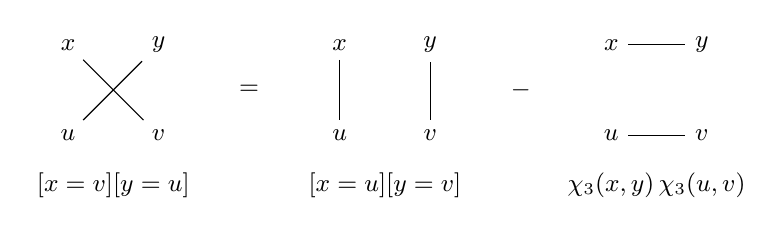
\begin{tikzpicture}[x=1.15cm,y=1.15cm,every node/.style={font=\small}]
\foreach \X/\T in {0/{$[x=v][y=u]$},3/{$[x=u][y=v]$},6/{$\chi_3(x,y)\,\chi_3(u,v)$}}{
  \node at (\X+0.5,-0.55) {\T};
  \node (x\X) at (\X,1) {$x$};
  \node (y\X) at (\X+1,1) {$y$};
  \node (u\X) at (\X,0) {$u$};
  \node (v\X) at (\X+1,0) {$v$};
}
\draw (x0)--(v0); \draw (y0)--(u0);
\draw (x3)--(u3); \draw (y3)--(v3);
\draw (x6)--(y6); \draw (u6)--(v6);
\node at (2,0.5) {$=$}; \node at (5,0.5) {$-$};
\end{tikzpicture}
\end{center}

A product $g(x,u)g'(y,v)$ is \emph{across the columns}: one factor reads only the column $b$, and the other only the column $b'$. A product $g(x,y)g'(u,v)$ is \emph{across the rows}. So $U$ is one product across the columns, and $S$ is one product across the rows. Thus~\eqref{identity} replaces two wires that survive both merges by $U$, which needs no wire between the two columns once they are merged, and $S$, which needs no wire between the two rows once they are merged. In the example, multiply~\eqref{identity} by $F_0(x)F_1(y)F_2(u)F_3(v)$ and sum over the four bits:
\begin{align*}
35&=\Bigl(\sum_xF_0(x)F_2(x)\Bigr)\Bigl(\sum_yF_1(y)F_3(y)\Bigr)-\Bigl(\sum_{x,y}F_0(x)F_1(y)\chi_3(x,y)\Bigr)\Bigl(\sum_{u,v}F_2(u)F_3(v)\chi_3(u,v)\Bigr)\\
&=12\cdot4-(-1)(-13)=48-13.
\end{align*}
Here $48$ is a product over the two columns, and $13$ is a product over the two rows.

\emph{Many wires.} A rectangle can carry many wires. Let $x,y,u,v$ be numbers of $m$ bits, with bits $x_j,y_j,u_j,v_j$ for $0\le j<m$, and let $U_j,S_j$ be $U,S$ at the position $j$. By~\eqref{identity}, the crossing $[x=v][y=u]$ is $\prod_j(U_j-S_j)$. Multiplied out, this is a sum of $2^m$ products, one for each set $T$ of positions that take $-S_j$. If each product became its own term, the number of terms of a network would be exponential in its number of wires. With two terms per rectangle, that number depends only on the grid. So we group the products by the size of $T$, into two \emph{pieces}:
\[
P^{\mathrm r}=\sum_{|T|\ge m/2}\ \prod_{j\in T}(-S_j)\prod_{j\notin T}U_j,\qquad P^{\mathrm c}=\sum_{|T|<m/2}\ \prod_{j\in T}(-S_j)\prod_{j\notin T}U_j,\qquad P^{\mathrm r}+P^{\mathrm c}=[x=v][y=u].
\]
For $m=1$ this is~\eqref{identity}: $P^{\mathrm r}=-S$ and $P^{\mathrm c}=U$, which contribute $-13$ and $48$ in the example.

A piece costs new wires. Suppose a piece is a sum of products across the rows, over an index $\xi$ of $d$ bits. In Section~3, $\xi$ becomes $d$ wires between the two rows, in place of the $2m$ wires of the crossing; the same holds for the columns. So our goal is $d<2m$, for $P^{\mathrm r}$ across the rows and for $P^{\mathrm c}$ across the columns (Lemma~\ref{lem:seed}). For this we expand $U_j$ and $S_j$ both ways. We need two more functions of two bits,
\[
\chi_1(p,q)=\tfrac12(1-\hat p\hat q)=[p\ne q],\qquad\chi_2(p,q)=\tfrac12(\hat p+\hat q)=[p=q]\hat p.
\]
Then, with $c$ running over $0,1,2,3$,
\begin{align*}
2U_j&=\sum_{c}\chi_c(x_j,y_j)\chi_c(u_j,v_j),\\
2S_j&=\chi_0(x_j,u_j)\chi_0(y_j,v_j)-\chi_1(x_j,u_j)\chi_1(y_j,v_j)-\chi_2(x_j,u_j)\chi_2(y_j,v_j)+\chi_3(x_j,u_j)\chi_3(y_j,v_j).
\end{align*}
To check the first line, add in pairs: the terms $c=0,1$ give $\tfrac12(1+\hat x_j\hat y_j\hat u_j\hat v_j)$, and the terms $c=2,3$ give $\tfrac12(\hat x_j\hat u_j+\hat y_j\hat v_j)$. In the second line, the terms $c=0,1$ give $\tfrac12(\hat x_j\hat u_j+\hat y_j\hat v_j)$, and the terms $c=2,3$ give $-\tfrac12(\hat x_j\hat v_j+\hat y_j\hat u_j)$. A \emph{string} is an element $\pi$ of $\{0,1,2,3\}^m$. Let $f_\pi(p,q)=\prod_j\chi_{\pi_j}(p_j,q_j)$ for numbers $p,q$ of $m$ bits, and let $n_c(\pi)$ be the number of letters $c$ of $\pi$.

\begin{lemma}\label{lem:seed}
Let $m=0$, or let $m=2k+1$ be odd. Put $\beta_0=0$ and $\beta_{2k+1}=2k+1+\lceil8k/5\rceil$. Then $\beta_m<2m$ for odd $m$, because $\lceil8k/5\rceil\le2k$. Each of $P^{\mathrm r},P^{\mathrm c}$ is a sum over an index $\xi$ of products $g_\xi(x,y)g'_\xi(u,v)$ (across the rows), and also a sum over an index $\xi$ of products $g_\xi(x,u)g'_\xi(y,v)$ (across the columns). The index has this number of bits:
\begin{center}
\begin{tabular}{l|cc}
 & across the rows & across the columns\\\hline
$P^{\mathrm r}$ & $\beta_m$ & $2m$\\
$P^{\mathrm c}$ & $2m$ & $\beta_m$
\end{tabular}
\end{center}
All values are dyadic with $O(m+1)$ bits, and they are computed in time polynomial in $m$.
\end{lemma}

\begin{proof}
For $m=0$ there is only $T=\varnothing$, so $P^{\mathrm r}=1$ and $P^{\mathrm c}=0$. Let $m=2k+1$. Fix $T$ and multiply out the expansions at each position.

\emph{Across the rows.} At $j\in T$ we have $-S_j=-\chi_3(x_j,y_j)\chi_3(u_j,v_j)$, and at $j\notin T$ we have $U_j=\frac12\sum_c\chi_c(x_j,y_j)\chi_c(u_j,v_j)$. So the product of $T$ is $(-1)^{|T|}2^{|T|-m}$ times the sum of $f_\pi(x,y)f_\pi(u,v)$ over the strings $\pi$ with the letter $3$ on all of $T$.

\emph{Across the columns.} At $j\notin T$ we have $U_j=\chi_0(x_j,u_j)\chi_0(y_j,v_j)$, and at $j\in T$ we have $-S_j=\frac12\bigl(-\chi_0\chi_0+\chi_1\chi_1+\chi_2\chi_2-\chi_3\chi_3\bigr)$, each factor at $(x_j,u_j)$ and $(y_j,v_j)$. So the product of $T$ is $2^{-|T|}$ times a signed sum of $f_\pi(x,u)f_\pi(y,v)$ over the strings $\pi$ with the letter $0$ off $T$.

So each piece is, across either cut, a sum over $\pi$ of a number $c_\pi$ times $f_\pi f_\pi$. For a string $\pi$, a set $T$ that fits it contributes a sign and a power of two that depend only on $|T|$ and on $\pi$, and the number of fitting sets of size $i$ is $\binom{n_3(\pi)}{i}$ across the rows and $\binom{n_0(\pi)}{i-m+n_0(\pi)}$ across the columns. So $c_\pi$ is a sum of at most $m+1$ numbers, each a binomial times a power of two with a sign. For $2m$ bits, the index names $\pi$ with two bits per letter; then $g_\xi=c_\pi f_\pi$ and $g'_\xi=f_\pi$.

For $\beta_m$ bits: a set $T$ of $P^{\mathrm r}$ has $|T|\ge k+1$, so across the rows only strings with at most $k$ letters other than $3$ occur. A set $T$ of $P^{\mathrm c}$ has $|T|\le k$, so across the columns only strings with at most $k$ letters other than $0$ occur. Each of these other letters has three values. So the first $m$ bits of the index mark the positions of the special letter ($3$ for $P^{\mathrm r}$, $0$ for $P^{\mathrm c}$), and the other $\lceil8k/5\rceil$ bits hold a number below $3^k$, whose base $3$ digits are the other letters, in order. Indexes that do not arise get the zero function. The number fits because $3^{5k}=243^k\le256^k=2^{8k}\le2^{5\lceil8k/5\rceil}$.
\end{proof}

\section{One step}\label{sec:step}

Section~2 treats one rectangle. A network has wires on many pairs of nodes. We now apply the split to all rectangles at once and then merge nodes, so that the value becomes a sum of values of networks with $K'$ nodes.

Let $(K'K',w,F)$ be a network. Two rows $a<a'$ and two columns $b<b'$ define a rectangle $\rho$. Its \emph{diagonals} are the pairs of nodes $\{(a,b),(a',b')\}$ and $\{(a,b'),(a',b)\}$. Each pair of nodes in different rows and different columns is a diagonal of exactly one rectangle. Let $w_1,w_2$ be the weights of the two diagonals of $\rho$, and let $m_\rho$ be the largest odd number at most $\min(w_1,w_2)$, or $0$ if the minimum is $0$. (Lemma~\ref{lem:seed} takes $m$ odd or $0$. An even $m$ would save nothing at $m=2$: the index would have $2+\lceil8/5\rceil=4=2m$ bits.) The lowest $m_\rho$ bits of the numbers on the two diagonals are the \emph{paired} bits: with the numbers
\[
x=B((a,b),(a',b')),\quad v=B((a',b'),(a,b)),\quad y=B((a,b'),(a',b)),\quad u=B((a',b),(a,b')),
\]
taken modulo $2^{m_\rho}$, the condition that the paired bits agree is the crossing $[x=v][y=u]$ of Section~2. A pair of nodes that is not a diagonal of a rectangle has no paired bits. All other bits of a number are its \emph{carried} bits.

\emph{Choices.} A \emph{choice} $\sigma$ picks, for each rectangle $\rho$, one of the two pieces $P_\rho\in\{P^{\mathrm r},P^{\mathrm c}\}$ of its crossing. There are $(K'(K'-1)/2)^2\le K'^4/4$ rectangles, so at most $2^{K'^4/4}$ choices. Fix $B$. The test $[B(s,t)=B(t,s)]$ says that the carried bits agree and the paired bits agree. Over all pairs of nodes, the tests of the paired bits multiply to $\prod_\rho[x=v][y=u]=\prod_\rho(P^{\mathrm r}+P^{\mathrm c})$, at the numbers $x,y,u,v$ of each $\rho$. Multiplying out this product gives one term for each $\sigma$:
\begin{equation}\label{expand}
\prod_{s,t}[B(s,t)=B(t,s)]=\sum_\sigma\ \prod_{s,t}[\text{the carried bits of $B(s,t)$ and $B(t,s)$ agree}]\ \prod_\rho P_\rho.
\end{equation}

\emph{Keeping the rows.} Fix $\sigma$. We build a network on the $K'$ rows. All numbers on the nodes of one row will be summed inside one new node function. So the wires inside a row disappear, and only what joins two rows must stay a wire. For a rectangle $\rho$, let $d^{\mathrm r}_\rho$ be $\beta_{m_\rho}$ if $P_\rho=P^{\mathrm r}$, and $2m_\rho$ if $P_\rho=P^{\mathrm c}$; by Lemma~\ref{lem:seed}, $P_\rho=\sum_\xi g_\xi(x,y)g'_\xi(u,v)$ with an index of $d^{\mathrm r}_\rho$ bits. For rows $a<a'$, the new wires between $a$ and $a'$, and what the new nodes do with them, are:
\begin{itemize}\setlength{\itemsep}{0pt}
\item for all columns $b,b'$, a copy of the carried bits of the number between $(a,b)$ and $(a',b')$. The node $a$ tests that this copy equals the carried bits of $B((a,b),(a',b'))$. The node $a'$ tests that it equals the carried bits of $B((a',b'),(a,b))$;
\item for all rectangles $\rho$ with these rows, the $d^{\mathrm r}_\rho$ bits of the index $\xi$ of $\rho$. The node $a$ has the factor $g_\xi(x,y)$, and the node $a'$ has the factor $g'_\xi(u,v)$.
\end{itemize}
So the new weight is
\begin{equation}\label{wrow}
w^{\mathrm r}(a,a')=\sum_bw((a,b),(a',b))+\sum_{b<b'}f^{\mathrm r}_\rho,\qquad f^{\mathrm r}_\rho=w_1+w_2-2m_\rho+d^{\mathrm r}_\rho,
\end{equation}
where $\rho$ is the rectangle with the rows $a,a'$ and the columns $b,b'$, and $w_1,w_2$ are the weights of its diagonals: $f^{\mathrm r}_\rho$ counts the carried bits on its diagonals and the bits of its index. Also $w^{\mathrm r}(a,a)=0$. The new node function at the row $a$ reads the family $B'$ of new numbers at $a$, and sums over the old numbers on all nodes of the row $a$:
\begin{equation}\label{newF}
F^{\mathrm r}_a(B')=\sum_{B}\ \mathsf T_a\ \prod_{b}F_{(a,b)}(B((a,b),\cdot)),
\end{equation}
where $B$ runs over the numbers $B(s,t)<2^{w(s,t)}$ for the nodes $s$ of the row $a$ and all nodes $t$. Here $\mathsf T_a$ is the product of the tests and factors of the node $a$ in the list above, for all other rows, and of the tests $B(s,t)=B(t,s)$ for two nodes $s,t$ of the row $a$. All of these read only numbers on the row $a$.

\emph{Keeping the columns.} Exchanging rows and columns gives a network $(K',w^{\mathrm c},F^{\mathrm c})$ on the columns: now the factors of a rectangle are across the columns, $g_\xi(x,u)$ and $g'_\xi(y,v)$; $d^{\mathrm c}_\rho$ is $\beta_{m_\rho}$ if $P_\rho=P^{\mathrm c}$, and $2m_\rho$ if $P_\rho=P^{\mathrm r}$; and $f^{\mathrm c}_\rho=w_1+w_2-2m_\rho+d^{\mathrm c}_\rho$.

\begin{lemma}\label{lem:step}
For each $\sigma$, pick the network on the rows or the network on the columns. Then $\val(K'K',w,F)$ is the sum over $\sigma$ of the values of the picked networks.
\end{lemma}

\begin{proof}
Consider the rows. Insert~\eqref{newF} in the value of the new network, multiply out the product over $a$ and reorder the sums. The value is the sum over all old $B$ of $\prod_sF_s(B(s,\cdot))$ times the sum of $\prod_aT_a$ over the new numbers; the tests of the new network leave one new number for each pair $a<a'$. Fix $B$. The new numbers are independent for different pairs $a<a'$, and each one splits into independent parts. A part that copies carried bits has two tests, one from each of the rows $a,a'$. Its sum is one test: the carried bits of $B(s,t)$ and $B(t,s)$ agree. The part of the index of $\rho$ has the sum $\sum_\xi g_\xi(x,y)g'_\xi(u,v)=P_\rho$. The tests inside a row are the tests of the carried bits for pairs in one row. So this sum is the summand of~\eqref{expand}, and the sum over $\sigma$ gives the product of all tests $[B(s,t)=B(t,s)]$. The columns are the same with the other expansion in Lemma~\ref{lem:seed}.
\end{proof}

\section{The potential}\label{sec:pot}

A rectangle with $P^{\mathrm r}$ has fewer new wires in the rows, and a rectangle with $P^{\mathrm c}$ has fewer in the columns. A choice may mix them, and a rectangle with $m_\rho=0$ keeps all its wires in both networks. So the number of wires need not fall. What does change is how the wires are spread over the pairs of nodes. In the network with $K'=2$ and $d$ wires between $(0,0)$ and $(1,1)$ only, the new network on the rows has $d$ wires between its two nodes. These wires occupied one pair of nodes out of six, and now they occupy the only pair. So we measure a network by a number that also sees the spread, the \emph{potential}
\[
\Phi(K,w)=K\Bigl(\sum_{s,t\in[K]}w(s,t)^2\Bigr)^{1/2}.
\]
For a fixed sum of weights, $\Phi$ is smallest when all pairs of nodes have the same weight, and then $\Phi$ is about twice the number of wires. In this network, $\Phi$ falls from $\sqrt{32}\,d$ to $\sqrt8\,d$ while the number of wires stays $d$. Cauchy over the $K^2$ ordered pairs of nodes gives
\begin{equation}\label{ends}
\sum_{s,t\in[K]}w(s,t)\le\Phi(K,w).
\end{equation}
The left side is the number of bits of a family $B$. So a small potential makes the sum over $B$ in $\val$ short. The potential falls by a fixed factor in one of the two networks:

\begin{lemma}\label{lem:phi}
Let $\gamma=\sqrt{24/25}$. For every $\sigma$,
$\min\bigl(\Phi(K',w^{\mathrm r}),\Phi(K',w^{\mathrm c})\bigr)\le\gamma\,\Phi(K'K',w)$.
\end{lemma}

\begin{proof}
Fix rows $a\ne a'$, and write each $f^{\mathrm r}_\rho$ in~\eqref{wrow} as $\frac12f^{\mathrm r}_\rho+\frac12f^{\mathrm r}_\rho$. Then~\eqref{wrow} has $K'+K'(K'-1)=K'^2$ terms, and Cauchy gives
\[
w^{\mathrm r}(a,a')^2\le K'^2\Bigl(\sum_{b<b'}\tfrac12(f^{\mathrm r}_\rho)^2+\sum_bw((a,b),(a',b))^2\Bigr).
\]
Sum over the ordered pairs $a\ne a'$ and multiply by $K'^2$. The left side becomes $\Phi(K',w^{\mathrm r})^2$. A rectangle arises from $(a,a')$ and from $(a',a)$, so the $\frac12$ disappears. The second sum becomes the sum over the ordered pairs of different nodes in one column. In the same way for the columns, so
\[
\Phi(K',w^{\mathrm r})^2+\Phi(K',w^{\mathrm c})^2\le K'^4\Bigl(\sum_{\rho}\bigl((f^{\mathrm r}_\rho)^2+(f^{\mathrm c}_\rho)^2\bigr)+\sum_{\substack{s\ne t\text{ in one row}\\\text{or one column}}}w(s,t)^2\Bigr).
\]
Fix $\rho$, with $w_1\ge w_2$, and $m=m_\rho$. One of $d^{\mathrm r}_\rho,d^{\mathrm c}_\rho$ is $2m$, which gives $f=w_1+w_2$. The other is $\beta_m$, which gives $f\le w_1+\frac9{10}w_2$. Indeed, if $m=0$ then $w_2=0$ and $f=w_1$. If $m=2k+1$ then $f-w_1=w_2-m+\lceil8k/5\rceil$ and $\lceil8k/5\rceil\le(8k+4)/5$, so $10(f-w_1)\le10(w_2-m)+16k+8$. Since $m$ is the largest odd number at most $w_2$, there are two cases: $w_2=2k+1$, where this bound is $16k+8\le9w_2$; and $w_2=2k+2$, where it is $16k+18\le9w_2$. So Cauchy gives
\[
(f^{\mathrm r}_\rho)^2+(f^{\mathrm c}_\rho)^2\le(w_1+w_2)^2+(w_1+\tfrac9{10}w_2)^2\le\bigl(2+1+\tfrac{81}{100}\bigr)(w_1^2+w_2^2)\le\tfrac{96}{25}(w_1^2+w_2^2).
\]
Each diagonal is two ordered pairs of nodes, so $w_1^2+w_2^2$ is half of the sum of $w(s,t)^2$ over the four ordered pairs of $\rho$. So the whole right side is at most $K'^4\cdot\frac{48}{25}\sum_{s,t}w(s,t)^2=\frac{48}{25}\Phi(K'K',w)^2$. The smaller of the two potentials has a square at most half of this. (Without the saving of Lemma~\ref{lem:seed} the constant $\frac{96}{25}$ would be $4$, and the potential would not fall.)
\end{proof}

\section{The chain of steps, and its cost}\label{sec:chain}

We now iterate until two nodes remain. Let $\ell\ge0$ and $K_j=2^{2^{\ell-j}}$, so that $K_0=2^{2^\ell}$, $K_\ell=2$ and $K_j=K_{j+1}K_{j+1}$.

\begin{theorem}\label{thm:net}
Let $(K_0,w,F)$ be a network, with potential $\Phi=\Phi(K_0,w)$. Then $\val(K_0,w,F)$ is computed in time $2^{K_0^2/3+4\gamma^\ell\Phi}$ times a constant depending on $\ell$, times a polynomial in $\Phi$ and the time and the bit length of one evaluation of a node function.
\end{theorem}

\begin{proof}
Put $N_0=(K_0,w,F)$. Given $N_j$ with $j<\ell$, pick a choice $\sigma_j$ for $N_j$, and let $N_{j+1}$ be the one of its two networks with the smaller potential, and the network on the rows if they are equal. A \emph{chain} is a sequence $(\sigma_0,\dots,\sigma_{\ell-1})$. By Lemma~\ref{lem:step}, $\val(N_0)$ is the sum of $\val(N_\ell)$ over all chains. By Lemma~\ref{lem:phi}, $N_j$ has potential at most $\gamma^j\Phi$.

The network $N_j$ has at most $K_{j+1}^4/4=K_j^2/4$ rectangles, and the next network has at most $K_{j+1}^2/4=K_j/4$, which is at most a quarter of $K_j^2/4$, since $K_j\ge4$. So all $N_j$ with $j<\ell$ have at most $K_0^2/3$ rectangles together, and there are at most $2^{K_0^2/3}$ chains.

Fix a chain. Computing all weights takes polynomial time, and it fixes which of the two networks is kept, since a comparison of potentials is a comparison of two sums of squares. By~\eqref{ends}, a family $B$ of $N_\ell$ has at most $\gamma^\ell\Phi$ bits, so the value of $N_\ell$ is a sum over at most $2^{\gamma^\ell\Phi}$ families $B$.

A node function of $N_{j+1}$ is~\eqref{newF}: a sum over the numbers $B((a,b),t)$ on one row of $N_j$, or on one column. Their number of bits is $\sum_b\sum_tw((a,b),t)$, a sum of $K_{j+1}^3$ weights $w$ of $N_j$. By Cauchy its square is at most $K_{j+1}^3\sum_{s,t}w(s,t)^2=\Phi(N_j)^2/K_{j+1}$, because $\Phi(N_j)^2=K_{j+1}^4\sum_{s,t}w(s,t)^2$. So these numbers have at most $E_j=\gamma^j\Phi/\sqrt{K_{j+1}}$ bits. Each term of the sum has one evaluation of $\mathsf T$ and $K_{j+1}$ evaluations of node functions of $N_j$. These evaluations are separate, so their costs add. So one evaluation of a node function of $N_\ell$ takes at most $\prod_{j<\ell}(K_{j+1}2^{E_j})$ evaluations of node functions of $N_0$, and as many evaluations of $\mathsf T$. For $r=\ell-j\ge1$ we have $\sqrt{K_{j+1}}=2^{2^{r-2}}\ge2^{r-1}$, so
\[
\sum_{j<\ell}E_j\le\gamma^\ell\Phi\sum_{r\ge1}\gamma^{-r}2^{1-r}=\frac{2\gamma^\ell\Phi}{2\gamma-1}\le3\gamma^\ell\Phi,
\]
since $\gamma\ge5/6$. Now multiply: there are at most $2^{K_0^2/3}$ chains; for one chain, the value of $N_\ell$ has at most $2^{\gamma^\ell\Phi}$ families and two evaluations of node functions of $N_\ell$ for each family; each of these takes at most $2^{3\gamma^\ell\Phi}\prod_{j<\ell}K_{j+1}$ evaluations of node functions of $N_0$ and of $\mathsf T$; and $\prod_{j<\ell}K_{j+1}$ is a constant depending on $\ell$. By Lemma~\ref{lem:seed}, $\mathsf T$ takes polynomial time. All numbers of wires are at most the number of wires of $N_0$, since $\beta_m\le2m$, and so at most $\Phi$. For the bits of values: if the values at level $j$ have at most $b_j$ bits, a value at level $j+1$ is a sum of at most $2^{E_j}$ products of at most $K_{j+1}$ values and of the factors of Lemma~\ref{lem:seed}, so $b_{j+1}\le E_j+K_{j+1}b_j+O\bigl(\sum_\rho(m_\rho+1)\bigr)$, with a constant depending on $\ell$. Hence $b_\ell$ is at most a constant times $b_0+\Phi+1$, and all values are dyadic with polynomially many bits.
\end{proof}

A chain also connects to OpenAI's partitions. Write a node of the first network as a string of $2^\ell$ bits. A row or a column keeps one half of these bits, so a chain selects one bit position, and the two nodes of the last network are the two groups of nodes with that bit fixed; compare the partitions in~\cite[Sections~2.4 and~2.7]{OAI26}, which are into small groups of variables. The sum over a group is not an enumeration here: the proof above evaluates it as nested sums, row by row. On one nested call path, the active summation indices have at most $\gamma^\ell\Phi+\sum_jE_j\le4\gamma^\ell\Phi$ bits.

For comparison, enumerating the bits of all wires costs $2^{\#\text{wires}}$, and the number of wires can be close to $\Phi/2$. The theorem replaces this exponent by $4\gamma^\ell\Phi$, at the cost of a factor $2^{K_0^2/3}$ that does not depend on the wires.

\section{Placing a formula}\label{sec:place}

Theorem~\ref{thm:net} helps when $\Phi=O(n)$. This holds if a formula has $O(n)$ occurrences and they are spread evenly over the pairs of nodes. A clause is a set of literals without a variable and its negation, and a formula is a set of clauses. An \emph{occurrence} is a pair $(i,C)$ of a variable $i$ and a clause $C$ containing it.

\begin{lemma}\label{lem:count}
Let $\ell\ge0$, $K=2^{2^\ell}$, $\Delta\ge3$. Let $\Psi$ be a formula with at most three literals per clause, on $n$ variables, each occurring at most $\Delta$ times. Then the number of assignments of the variables that occur, which satisfy $\Psi$, is computed in time $2^{16\Delta\gamma^\ell n}$ times a constant depending on $\ell$ and $\Delta$, times a polynomial in $n+\Delta$. It is positive if and only if $\Psi$ has a solution.
\end{lemma}

\begin{proof}
There are at most $\Delta n$ occurrences. \emph{Placement.} We want few occurrences on each pair of nodes. Number the variables $0,\dots,n-1$, and put them on the nodes cyclically: $\omega(i)$ is $i$ modulo $K$. A node holds at most $(n+K)/K$ variables, hence at most $\Delta(n+K)/K$ occurrences of its variables. Go through the clauses in any order, and let $\mathrm{load}(s,t)$ count the occurrences $(i,C)$ placed so far with $\omega(i)=s$ and $\omega(C)=t$. Put the clause $C$ on the node $t$ that minimizes $\sum_{i\in C}\mathrm{load}(\omega(i),t)$. For each $s$, $\sum_t\mathrm{load}(s,t)\le\Delta(n+K)/K$, and $C$ has at most three variables. So the minimized quantity, summed over all $K$ nodes $t$, is at most $3\Delta(n+K)/K$, and its minimum is at most $3\Delta(n+K)/K^2$. Placing $C$ raises a load by at most $3\le\Delta$. So all loads stay at most $\kappa=\Delta(3n+4K^2)/K^2$, using $K\le K^2$.

\emph{Network.} Each occurrence $o=(i,C)$ is a wire between $\omega(i)$ and $\omega(C)$, with one bit $\theta_o$. Number the wires between two nodes, so that $\theta_o$ is one bit of $B(\omega(i),\omega(C))$. The node function $F_s$ is the product of two kinds of tests. For a variable $i$ with $\omega(i)=s$, the test that $\theta_o$ is the same for all its occurrences $o$. For a clause $C$ with $\omega(C)=s$, the test that $C$ is true when each literal reads the bit of its occurrence. Then $\val(K,w,F)$ is the number in the statement.

\emph{Potential.} We have $w(s,t)\le\mathrm{load}(s,t)+\mathrm{load}(t,s)\le2\kappa$. So $\sum_{s,t}w(s,t)^2\le2\kappa\sum_{s,t}w(s,t)\le2\kappa\cdot2\Delta n$, and
\[
\Phi(K,w)^2\le K^2\cdot2\kappa\cdot2\Delta n=4\Delta^2n(3n+4K^2)\le\bigl(4\Delta(n+K^2)\bigr)^2.
\]
Theorem~\ref{thm:net} gives time $2^{K^2/3+16\Delta\gamma^\ell(n+K^2)}$ times a constant and a polynomial, and the terms with $K^2$ are a constant depending on $\ell$ and $\Delta$. The node functions take polynomial time.
\end{proof}

\section{Few occurrences, and the end of the proof}\label{sec:end}

A 3-CNF can have about $n^3$ clauses, and Lemma~\ref{lem:count} needs few occurrences per variable. Branching provides this. It is the sparsification of~\cite{IPZ01}, in a short form. A clause is a \emph{unit}, \emph{binary} or \emph{ternary} if it has $1$, $2$ or $3$ literals. To \emph{normalize} a formula, delete every clause that properly contains another clause; this keeps the set of solutions.

\begin{lemma}\label{lem:branch}
Let $q\ge2$, and let $\Psi$ be a formula on $n$ variables in which every clause is ternary. There is a binary tree with at most $\mathrm e^{(20\ln q+10)n/q}$ leaves, computed in polynomial time per vertex, whose leaves are formulas such that the solutions of $\Psi$ are the union of the solutions of the leaves, and in each leaf a variable occurs at most $4q^2$ times.
\end{lemma}

\begin{proof}
The root is $\Psi$. At a vertex, take the first case that applies, with ties broken lexicographically: (i) a literal lies in at least $q$ binaries; (ii) a pair of literals lies in at least $q$ ternaries; (iii) a literal lies in at least $q^2$ ternaries. If no case applies, the vertex is a leaf. Otherwise let $Z$ be that literal or pair, and write all those clauses as $Z\vee Y_1,\dots,Z\vee Y_J$. Since $\bigwedge_i(Z\vee Y_i)$ is equivalent to $Z\vee\bigwedge_iY_i$, every solution satisfies the clause $Z$ or all clauses $Y_i$. So the vertex has two children, whose solutions together are those of the vertex: the \emph{first child} adds the clause $Z$, the \emph{second child} adds all clauses $Y_i$, and both are normalized. At a leaf a literal lies in at most $1+(q-1)+(q^2-1)$ clauses, so a variable occurs at most $2(q^2+q-1)\le4q^2$ times.

It remains to count the leaves. For a vertex, let $\mu=3q\cdot\#\text{units}+\#\text{binaries}$; the root has $\mu=0$. We will show that $\mu\le8nq$ at every vertex, that $\mu$ rises by at least $1$ from a vertex to its first child, and that it rises by at least $q^2$ to its second child. This needs two facts about clauses.

\emph{Normalization deletes no added clause.} An added clause is new and contains no existing clause; otherwise $Z\vee Y_i$ would properly contain an existing clause and would have been deleted. The added $Y_i$ are distinct and of equal size, so none contains another.

\emph{At every vertex, every literal lies in fewer than $2q$ binaries.} The root has no binaries. Case (i) adds only units. In case (ii), every literal lies in fewer than $q$ binaries, since case (i) does not apply, and the vertex adds at most one binary. In case (iii), the same holds before the addition, and a literal $\nu$ lies in as many added $Y_i$ as there are ternaries containing the pair $\{Z,\nu\}$, which is fewer than $q$, since case (ii) does not apply.

\emph{Measure.} There are at most $2n$ units, and fewer than $2nq$ binaries by the bound above. So $\mu\le8nq$. A new unit adds $3q$ to $\mu$ and deletes fewer than $2q$ binaries, so $J$ new units raise $\mu$ by at least $J(q+1)$. A new binary adds $1$ and deletes only ternaries. Hence the first child raises $\mu$ by at least $1$. The second child raises $\mu$ by at least $q^2$: in cases (i) and (ii) it adds $J\ge q$ units, which raise $\mu$ by at least $q(q+1)$, and in case (iii) it adds $J\ge q^2$ binaries.

\emph{Leaves.} So a path from the root has at most $M=8nq$ edges, and at most $M/q^2=8n/q$ of them lead to a second child. Two leaves have different sets of positions of second children, because at the vertex where their paths part exactly one takes the second child. So the number of leaves is at most
\[
\sum_{i\le M/q^2}\binom Mi\le q^{2M/q^2}\sum_i\binom Miq^{-2i}=q^{2M/q^2}(1+q^{-2})^M\le q^{2M/q^2}\mathrm e^{M/q^2}=\mathrm e^{(16\ln q+8)n/q}.
\]
This is at most the bound in the statement, because $16\ln q+8\le20\ln q+10$; we state the weaker bound because Lean proves that one. A formula on a vertex has polynomially many clauses, because ternary clauses are only deleted and $\mu\le8nq$. So each vertex takes polynomial time.
\end{proof}

\begin{proof}[Proof of Theorem~\ref{thm:sat}]
The parameters depend on $\varepsilon$ only. Let $q\ge2$ be the least integer with $(20\ln q+10)/(q\ln2)\le\varepsilon/3$. Let $\ell$ be the least integer with $64q^2\gamma^\ell\le2\varepsilon/3$. These exist because the left sides tend to $0$. Put $\Delta=4q^2$.

The algorithm rejects an input with an empty clause, and deletes tautologies and repeated literals. Using two new variables $h,h'$, it replaces a binary clause $Y$ by $Y\vee h$, $Y\vee\neg h$, and a unit clause $Y$ by the four clauses $Y\vee h^{\pm}\vee h'^{\pm}$. This keeps satisfiability and raises $n$ by at most $2$, which changes the final bound by the constant factor $2^{2\varepsilon}$. Then it traverses the tree of Lemma~\ref{lem:branch}, and it uses Lemma~\ref{lem:count} at each leaf. It accepts if and only if some leaf has a solution. This is correct because the solutions of the formula are the union of those of the leaves.

The tree has at most $\mathrm e^{(20\ln q+10)n/q}\le2^{\varepsilon n/3}$ leaves, and at most twice as many vertices. Up to a constant and a polynomial factor, one leaf costs at most $2^{16\Delta\gamma^\ell n}$ by Lemma~\ref{lem:count}, and $16\Delta\gamma^\ell=64q^2\gamma^\ell\le2\varepsilon/3$. So the total time is at most a constant times $2^{\varepsilon n}$ times a polynomial in the input size, since the input declares its $n$ variables, so $n\le|\varphi|$.
\end{proof}

\section{Formalization}\label{sec:formal}

The Lean~4 development~\cite{Lean4,Mathlib} is the library \lean{UncrossingWires} in the directory \texttt{lean/} of the repository \url{https://github.com/suquark/NotETHSimplified}. It uses the libraries \lean{TransposeBase} and \lean{SatBase} of that project for the word language, helpers for brute force, binomials and fields, the network of a formula, the branching tree and the arithmetic choice of its parameter, and the machine layer, and \lean{FormalizationKit} for resource bounds on the machine. The file \lean{UncrossingWires/Audit.lean} reports that the theorems listed there depend only on the axioms \lean{propext}, \lean{Classical.choice} and \lean{Quot.sound}, or on a subset of them, and the library contains no \lean{sorry}. A meta-program, \lean{UncrossingWires/ClosureCheck.lean}, computes that closure, and it counts no constant with a name containing \lean{OnePigeonhole}, \lean{Chebyshev}, \lean{Fourier}, \lean{fourier}, \lean{Hermite}, \lean{indow}, \lean{Matrix.det}, \lean{.det} or \lean{det\_}. Table~\ref{tab:lean} maps the paper to the Lean declarations.

\begin{table}[ht]
\centering
\small
\resizebox{\textwidth}{!}{\begin{tabular}{@{}lll@{}}
\toprule
\textbf{Paper} & \textbf{Lean declaration} & \textbf{Module} \\
\midrule
Lemma~\ref{lem:seed} & \lean{Ppol\_add}, \lean{seed\_sum}, \lean{dLen\_le} & \lean{Seed} \\
Lemma~\ref{lem:step} & \lean{step\_val} & \lean{Step} \\
Lemma~\ref{lem:phi} & \lean{dLen\_cheap\_le}, \lean{potential\_two}, \lean{potential\_min} & \lean{Seed}, \lean{Potential} \\
Theorem~\ref{thm:net} & \lean{chain\_val}, \lean{chainVal\_eq}, \lean{core\_spec} & \lean{Chain}, \lean{Pseudo.CoreSpec} \\
Lemma~\ref{lem:count} & \lean{load\_table\_le}, \lean{psi\_table\_le\_all}, \lean{BaseNet.val\_base} & \lean{Greedy}, \lean{Base} \\
Lemma~\ref{lem:branch} & \lean{sparseTree\_leaves}, \lean{noSparseRule\_variable\_bound} & \lean{SatBase} \\
Theorem~\ref{thm:sat} & \lean{Pseudo.Final.pseudo\_main}, \lean{Machine.not\_ETH} & \lean{Pseudo.Final}, \lean{Machine.FinalMain} \\
\bottomrule
\end{tabular}}
\caption{Map from the paper to the Lean development. Names are in \lean{UncrossingWires} except those of Lemma~\ref{lem:branch}, in \lean{SatBase}.}\label{tab:lean}
\end{table}

The Lean proof departs from the text in these ways. The node functions are integers, with a fixed power of two for each rectangle. Each variable has one more wire, to a node of its own, because Lean counts the assignments of all $n$ variables, and the text those of the variables that occur. A choice is encoded in $K'^4$ bits with a validity test, not in $K'^4/4$ bits. The potential bound of Lemma~\ref{lem:count} is \lean{psi\_table\_le\_all}, for every $n$. The program instead enumerates small $n$ at the root, for $n\le K^2$, and uses the sharper bound \lean{psi\_table\_le} for larger $n$; the text has no enumeration. Clauses are sets of literals that may hold both signs of a variable, and clauses of fewer than three literals are allowed, with no padding, no new variables and no deletion of tautologies. The tree of Lemma~\ref{lem:branch} is the same, and Lean proves its statement with another measure, in \lean{sparseTree\_leaves} and \lean{noSparseRule\_variable\_bound}. The constants of Theorem~\ref{thm:sat} are computed by hand here, and Lean has its own: \lean{exists\_rate} uses a rate $(49/50)^H$, with $(49/50)^2\ge24/25$.

\medskip\noindent\emph{The algorithm.} The word language has addition, subtraction and multiplication modulo $2^{\mathsf w}$, division, remainder, powers of $2$, comparison, and bounded loops. Its semantics gives the value of a program and the number of word operations, counted over the iterations that actually run. The theorem \lean{Pseudo.Final.pseudo\_main} states: for every $\varepsilon>0$ there are one program $\mathsf P$ and constants $C,b,c$ such that for every $n$ and every formula $F$ with $n$ variables and clauses of at most three literals, with $\mathsf w=c(n+1)^3$ and input the bitset of $F$ and the number $n$, the value of $\mathsf P$ is nonzero exactly when $F$ is satisfiable, and the number of word operations is at most $C(n+1)^b2^{\varepsilon n}$. The first-level tables are bound as words; a later level has a constant number of nodes, and its weights are recomputed by nested expressions from the code of the chain. The theorem \lean{Pseudo.core\_spec} gives the value and the cost of one network.

\medskip\noindent\emph{The machine.} The compiler \lean{compile\_correct} of \lean{TransposeBase} compiles every program of this language to a program on Boolean stacks, with a time of at most $7000(\mathsf w+1)^2$ source instructions for each word operation, and a bound of $7100(\mathsf w+1)^2$ bits on every stack at every prefix. Together with a parser of the input, and a compiler to a primitive multitape machine of OpenAI~\cite{OAIlean}, whose code is included in \texttt{lean/third\_party/} with its license and a patch record, this gives \lean{Machine.machine\_main}: for every $\varepsilon>0$ there are a primitive machine and constants such that, for every $n$ and every formula $\varphi$ with $n$ variables and clauses of at most three literals, the machine started on the fixed encoding of $\varphi$ halts with the answer, in at most $C(|\varphi|+1)^d2^{\varepsilon n}$ steps, where $|\varphi|$ is the length of the encoding; and every prefix of that same run visits at most $C'(|\varphi|+1)^{d'}$ tape cells. The word width there is $\mathsf w=c(|\varphi|+1)^4+|\varphi|$. The theorem \lean{Machine.not\_ETH} states the failure of ETH in this model. These theorems have the form that refuting ETH requires: a machine for each $\varepsilon$. One algorithm with running time $2^{o(n)}$ is a stronger statement, which Lean does not state. The file \lean{UncrossingWires/Audit.lean} checks by \lean{rfl} that these end statements coincide with those of \lean{TransposeBase}.

\medskip\noindent\emph{What is not formalized.} Theorem~\ref{thm:net} is stated in Lean only as \lean{Pseudo.core\_spec}, for placed networks with one bit per wire, in word operations, with its exponent as an unsummed sum of the $E_j$ and $\gamma^\ell\Phi$. The value part, \lean{chain\_val}, holds for arbitrary symmetric weights. The proof of Lemma~\ref{lem:branch} with the measure $\mu$ and the constants of this text are not formalized. The script \texttt{checks/check\_step.py} in the directory of this paper tests the identity and the expansions, the pieces with their coefficients, Lemma~\ref{lem:step} in Lean's integer form, and the single-rectangle inequality of Lemma~\ref{lem:phi}, exactly, on tiny networks, including two crossing rectangles for $K'=3$.

\section*{Use of AI}
The argument and the Lean proofs were developed in interactive sessions with Claude (Anthropic), building on the public manuscripts~\cite{OAI26,OD26,Cla26,Kin26}. The author is responsible for any errors.

\begin{thebibliography}{IPZ01}
\bibitem[Cla26]{Cla26} Claude (Anthropic). A $2^{o(n)}$ time algorithm for 3-SAT. Preprint, October 26, 2026. \url{https://github.com/anthropics/formal-math/tree/16a5ce41304fcdaea4e0be7c132e1c361dc26da5/eth}.
\bibitem[ETH26]{ETHblog} R.~Impagliazzo, R.~Paturi, and R.~Williams. ETH refutation: examination and discussion. Web site, October 2026. \url{https://ethdiscussion.blog/2026/10/26/eth-refutation-examination-and-discussion/}.
\bibitem[IP01]{IP01} R.~Impagliazzo and R.~Paturi. On the complexity of $k$-SAT. \emph{J.\ Comput.\ System Sci.} 62(2):367--375, 2001.
\bibitem[IPZ01]{IPZ01} R.~Impagliazzo, R.~Paturi, and F.~Zane. Which problems have strongly exponential complexity? \emph{J.\ Comput.\ System Sci.} 63(4):512--530, 2001.
\bibitem[Kin26]{Kin26} S.~Kintali. A simplified proof of ETH is false. Manuscript, October 26, 2026. \url{https://shivakintali.github.io/papers/ETH.pdf}.
\bibitem[MU21]{Lean4} L.~de Moura and S.~Ullrich. The Lean 4 theorem prover and programming language. In \emph{Proc.\ 28th CADE}, 2021.
\bibitem[mC20]{Mathlib} The mathlib Community. The Lean mathematical library. In \emph{Proc.\ 9th ACM SIGPLAN CPP}, 2020.
\bibitem[OAI26]{OAI26} OpenAI. The Exponential Time Hypothesis is false. Manuscript, October 17, 2026; revised October 25, 2026. \url{https://github.com/openai/math/blob/42907c9e999cc00d6abe7a50bfc1023250edd1b9/preprints/The-Exponential-Time-Hypothesis-is-False-October-25-2026/paper.pdf}.
\bibitem[OAI26b]{OAIlean} OpenAI. Lean formalization accompanying ``The Exponential Time Hypothesis is false''. Repository, commit 4eaee87; see \texttt{lean/OAI/Algorithms/SubexponentialSAT/SqrtLogSpace/CompileSpace.lean}. \url{https://github.com/openai/math/tree/4eaee87548250b2682affda7d05d947c05554bae/lean}.
\bibitem[O'D26]{OD26} R.~O'Donnell. Some exposition of ``The Exponential Time Hypothesis Is False''. Manuscript, October 30, 2026. \url{https://www.cs.cmu.edu/~odonnell/some_eth_false_exposition.pdf}.
\end{thebibliography}
\end{document}
